\documentclass[oneside]{report}
\usepackage[all]{xy}
\usepackage{amsmath,amsthm,amssymb,graphicx,tikz,fancyhdr,hyperref} 
\usepackage{graphicx,hyperref,fancyhdr,amsmath,amssymb,color,xspace}
\usepackage{fancyhdr}
\usepackage[extrafootnotefeatures]{xepersian}
\settextfont[Scale=1]{Yas}
\setdigitfont[Scale=1.1]{Yas}
\setlatintextfont{Times New Roman}
\linespread{1.8}
\newtheorem{dfn}{تعریف}
\newtheorem{thm}{قضیه}
\newtheorem{pro}{گزاره}
\newtheorem{rem}{تذکر}
\newtheorem{lem}{لم}
\newtheorem{cor}{فرع}
\newtheorem{ex}{مثال}
\newtheorem{qu}{سوال}
\newtheorem{con}{ساخت}
\renewenvironment{proof}{\noindent{\bf برهان. }  \rm }{\hfill{$\Box$}\\}
\renewcommand{\bibname}{مراجع}
\fancyhead[RE]{\thepage}
\fancyhead[LO]{\thepage}
\fancyfoot{\empty} 
\pagestyle{fancy}
\newcommand{\Lfootnote}[1]{\hspace{-1mm}\LTRfootnote{\rm #1}~}

\newtheorem{definition}{Definition}
%%%%%%%%%%%%%%%%%%%%%%%%%%%%  در ابتدا از نصب فونت Yas بر روی سیستم مطمئن شوید. %%%%%%%%%%%%%%%%%%%%%%%55
%%%%%%%%%%%%%%%%%%%% دستور رنگی کردن لینک‌ها %%%%%%%%%%%%%%%%%%%%%%%%%%%%%%%
\hypersetup{colorlinks=true,linkcolor=red,citecolor=blue,filecolor=magneta,urlcolor=cyan}
\begin{document}
\thispagestyle{empty}
%%%%%%%%%%%%%%%%% سربرگ (عنوان مقاله)  %%%%%%%%%%%%%%%%%%%%
\fancyhead[LE]{پروژهٔ ساخت بویایی‌سنج کنترل‌شونده با کامپیوتر}
%%%%%%%%%%%%%%%%% نویسندگان (عنوان مقاله)  %%%%%%%%%%%%%%%%%%%%
\fancyhead[RO]{پروژهٔ ساخت بویایی‌سنج کنترل‌شونده با کامپیوتر}
\begin{flushright}
\vspace*{4cm}
%%%%%%%%%%%%%%%%% عنوان مقاله  %%%%%%%%%%%%%%%%%%%%
{\Large \bf پروژهٔ ساخت بویایی‌سنج کنترل‌شونده با کامپیوتر}\\
%%%%%%%%%%%%%%%%% نویسندگان مقاله و نشانی %%%%%%%%%%%%%%%%%%%%
{\bf
امیرحسین افشارراد، محمد‌مهدی کیانی، بهراد منیری، هادی حجتی
}


هستهٔ پژوهشی هوش محیطی، دانشکدهٔ مهندسی برق، دانشگاه صنعتی شریف

\end{flushright}
\vspace {.5cm}

%%%%%%%%%%%%%%

\paragraphfootnotes
\section*{مقدمه}
حس بویایی یکی از حواس پنج گانهٔ انسان است که معمولا کمتر از سایر حس‌ها مورد توجه قرار می گیرد. حتی در زبان فارسی نیز فعلی برای دریافت و یا حس کردن بو وجود ندارد و بسیاری از افراد از فعل "شنیدن" به منظور اشاره کردن به فرآیند دریافت تحریک بویایی استفاده می کنند.
با این حال بویایی تاثیر قابل توجهی بر روی زندگی انسان و فعالیت‌های او دارد و مطالعهٔ آن خالی از فایده نیست؛ برای مثال بسیاری از ما با حس کردن یک بوی خاص به یاد خاطره‌ای خوش و یا فردی نزدیک در زندگی‌مان می‌افتیم و با حس‌کردن بویی دیگر خاطره و یا اتفاق تلخی را به یاد می‌آوریم. همچنین قرار‌گرفتن در محیطی با بوی نامطبوع موجب آزرده‌شدن افراد و حتی مختل شدن فعالیت هایشان می‌شود.


دانسته‌های ما از حس بویایی نسبت به سایر حس‌ها محدود‌تر است و هنوز پرسش‌های زیادی در مورد آن وجود دارد که دانشمندان درصدد پاسخ به آن هستند؛ برای مثال هنوز بر دانشمندان پوشیده است که آیا بینی تنها عضو دخیل برای دریافت تحریک‌های
بویایی است و یا چرا برخی بوها در برخی فرهنگ‌ها و یا برای برخی افراد مطبوع به شمار می‌آیند در حالی که برای افراد دیگر نامطبوع‌اند. همچنین عملکرد مغز در هنگام تشخیص بو و مرز میان جنبهٔ شیمیایی و روانشناسانهٔ بویایی هنوز قابل تفکیک نیست.


موضوعات زیادی در مورد حس بویایی وجود دارد که هنوز بر روی آن تحقیقات زیادی انجام نگرفته است؛ یکی از این موضوعات، عملکرد مغز در هنگام بویایی و واکنش آن به تحریک‌های مختلف بویایی است. روش‌های تصویر برداری مغزی همانند EEG و fMRI به دانشمندان این امکان را داده است تا نحوهٔ عملکرد مغز در موقعیت‌های مختلف را مورد بررسی قرار دهند. این پیشرفت‌ها به دانشمندان این امکان را داده تا در مورد حواسی مانند بینایی و شنوایی تحقیقات جامعی انجام دهند و تا حد زیادی به عملکرد مغز در هنگام استفاده از این حواس پی ببرند. با این حال برخلاف بینایی و شنوایی، دانشمندان زیادی بر روی ارتباط میان عملکرد مغز و حس بویایی تحقیق نکرده‌اند. یکی از مهم‌ترین دلایل این موضوع، دشواری به دست آوردن داده‌های مورد نیاز است. دادن تحریک بویایی نسبت به تحریک شنوایی و بینایی دشوارتر است و مشکلات زیاد مرتبط با آن باعث می شود تا داده‌های حاصل برای انجام تحقیق از دقت کافی برخوردار نباشند.



یکی از روش های مرسوم برای دادن تحریک بویایی که همچنان نیز در برخی از تحقیقات مورد استفاده قرار می گیرد، به این ترتیب است که آزمایش‌کننده اسانس با بوی مد نظر را داخل یک ظرف می ریزد و سپس آن را زیر بینی آزمایش‌شونده قرار داده و از او می خواهد تا نفس بکشد. این روش آزمایش ایرادات زیادی دارد؛


 نخستین مشکل آن است که در این آزمایش، زمان پخش بو از کنترل آزمایش‌شوندگان خارج است. برای مثال فرض کنید می خواهیم آزمایشی طراحی کنیم که در آن ابتدا بوی A به مدت 10 ثانیه پخش می شود، سپس 10 ثانیه بویی پخش نمی شود (حالت استراحت) و در نهایت بوی B برای آزمایش‌شونده پخش می‌گردد. در صورتی که این آزمایش را به روشی که پیش‌تر توضیح داده شد انجام دهیم، بوی A در حالت استراحت نیز در هوا می‌ماند و حتی ممکن است در صورت کوتاه بودن زمان استراحت، با بوی B نیز ترکیب شود. با کنترل‌کردن نرخ‌تنفس فرد و سنکرون کردن آن می‌توان این مشکل را تا حدی برطرف کرد. همچنین به منظور جلوگیری از ترکیب دو بو، میتوان زمان استراحت را طولانی‌تر نمود.


مشکل دوم این روش در آزمایش‌های بویایی آن است که ممکن است آزمایش‌شونده پیش از احساس تحریک‌بویایی، در مورد آن قضاوت کند. برای مثال آزمایش‌شونده از طریق مشاهدهٔ فعالیت‌های آزمایش‌کننده می‌تواند به عوض‌شدن بو و یا شروع زمان 
استراحت پی‌ببرد که موجب می‌شود نتایج حاصل، مطلوب ما نباشد. برای حل این مشکل نیز بسیاری از محققان آزمایش خود را به گونه‌ای طراحی نمودند که در طول آن چشم و گوش آزمایش‌شونده بسته بماند.

همانگونه که پیش‌تر گفته شد، این روش با وجود کاستی‌هایی که دارد همچنان در بسیاری از تحقیقات در مورد حس بویایی مورد استفاده قرار می‌گیرد و محققان می‌کوشند به کمک روش‌هایی که توضیح‌داده‌شده، خطای ناشی از عوامل مذکور را کمتر کنند.
با این حال آزمایش‌هایی وجود دارند که به کمک روش گفته شده قابل انجام نیستند و یا نتایج حاصل از آن‌ها با آنچه مطلوب ماست فاصلهٔ زیادی دارد. یکی از این آزمایش‌ها، آزمایش Oddball بویایی است. 

مرجع \cite{Kroupi} مثالی از این آزمایش هاست.

\section*{بویایی‌سنج}
مطالعه ی زیادی بر روی آزمایش Oddball برای تحریک‌های بینایی و شنوایی انجام شده است اما به دلیل مشکلات موجود در دادن تحریک بویایی، انجام این آزمایش به روشی که پیش‌تر گفته شد عملاً با مشکلات زیادی رو‌به‌رو خواهد‌بود. به منظور دادن تحریک Oddball بویایی، نیاز به دستگاهی داریم که بوها را کنترل‌شده و در مدت زمان معین به آزمایش‌شونده برساند. 
بدین منظور دستگاهی با نام  الفکتومتر یا بویایی‌سنج\LTRfootnote{Olfactometer}
 ساخته شده است. این دستگاه، تحریک بویایی را از طریق یک وسیله (معمولاً کامپیوتر) به آزمایش‌شونده می‌رساند. در سال‌های اخیر، چندین نوع الفکتومتر توسط محققان طراحی و ساخته شده است. تایلر لوریگ\LTRfootnote{Tyler S. Lorig}
 از دانشگاه واشنگتن اند لی\LTRfootnote{Washington and Lee University}
 در سال 1999 یک الفکتومتر طراحی کرد که تحریک بویایی را به کمک رله‌های کنترل‌شونده مطابق میل آزمایش کننده‌ها به آزمایش شونده می رساند \cite{Elmes}.
 از آن زمان تا‌کنون چندین محقق دیگر نیز به منظور انجام آزمایش‌های بویایی خود طرحی مشابه با طرح لوریگ طراحی کردند. برای مثال در سال 2006، استیون لوون و اسکات لوکاس از بیمارستان مک لارن و دانشگاه هاروارد طرحی برای ساخت الفکتومتر ارزان ارائه دارند و با حدود 400 دلار موفق به ساخت آن شدند \cite{Lowen}؛
 با این حال الفکتومتر ساخته‌شده توسط آن‌ها به دلیل تاخیر در رساندن تحریک‌بویایی، مناسب آزمایش Oddball نبود.
این محققان در سال 2016 طرح دیگری برای ساخت الفکتومتر ارائه دادند و این مشکل را برطرف نمودند که هزینهٔ تمام شدهٔ آن حدود 1100 دلار بود.

به عنوان یک مثال دیگر در همین زمینه، می‌توان به الفکتومتر طراحی شده توسط یوهان لوندستروم در سال 2010 اشاره کرد. این محقق و همکارانش تلاش کردند تا الفکتومتری طراحی کنند که در عین ارزان بودن، از لحاظ ساخت نیز راحت باشد. نتیجهٔ کار آنها ساخت الفکتومتری با حدود 5200 دلار بود و تمامی مراحل ساخت را نیز در مقالهٔ خود توضیح دادند \cite{Lunder}.
لازم به ذکر است علاوه بر الفکتومترهای ساخته شده توسط محققان، الفکتومترهای دیگری نیز وجود دارند که به صورت تجاری فروخته می‌شوند؛ با این حال قیمت بالای این دستگاه‌ها باعث می‌شود که بسیاری از محققان از خرید آن صرف نظر کنند و پژوهشگرانی که قصد مطالعه بر روی حس بویایی را دارند، ترجیح می‌دهند الفکتومتر خودشان را طراحی نمایند. علاوه بر این، تعداد شرکت‌های سازندهٔ این وسیله نیز بسیار محدود است و تهیهٔ آن علاوه بر هزینهٔ زیاد، مشکلات زیادی نیز در بر خواهد داشت.


این موضوعات ما را بر آن داشت تا الفکتومتری طراحی کنیم که ویژگی های زیر را داشته باشد:
\begin{enumerate}
\item
ارزان باشد؛ همانگونه که گفته شد پیش تر الفکتومترهایی ساخته‌شدند که هدف اصلی آنها این بود که هزینهٔ تمام‌شده حداقل باشد. ما نیز در طراحی خود می کوشیم تا این هدف محقق شود.
\item
مناسب برای انجام آزمایش Oddball باشد؛ بدین منظور، تاخیر بین دادن دستور به الفکتومتر و رسیدن تحریک بویایی به بینی آزمایش‌شونده باید حداقل باشد.
\item
مناسب برای انجام آزمایش‌های EEG و fMRI باشد؛ به منظور این که بتوانیم از این دستگاه در آزمایش های MRI استفاده کنیم، هیچ قطعه ی فلزی‌ای نباید در قسمتی از الفکتومتر که وارد دستگاه MRI می شود، قرار داشته‌باشد.
\item
خطری برای آزمایش شونده نداشته باشد؛ این دستگاه نباید به هیچ عنوان صدمه‌ای به دستگاه بویایی و تنفسی آزمایش‌شونده‌ها بزند.
\end{enumerate}



\section*{طراحی}

هوای مورد نیاز به وسیلهٔ یک کمپرسور به دستگاه داده می شود و جریان هوا را به کمک یک فلومتر اندازه می‌گیریم. در صورتی که جریان هوا بیش از 3 لیتر بر دقیقه باشد، آزمایش‌شونده با گذشت زمان دچار خشکی بینی می‌شود؛ همچنین کم بودن جریان نیز باعث می‌شود تا زمان رسیدن تحریک بویایی افزایش پیدا کند. به همین دلیل ما جریان هوا را در داخل دستگاه برابر 3 لیتر بر دقیقه قرار می‌دهیم تا نه موجب آزار آزمایش‌شونده شود و نه از دقت دستگاه بکاهد. شکل ۱ شماتیک کلی این دستگاه است.

\begin{figure}[h]
	\centering
	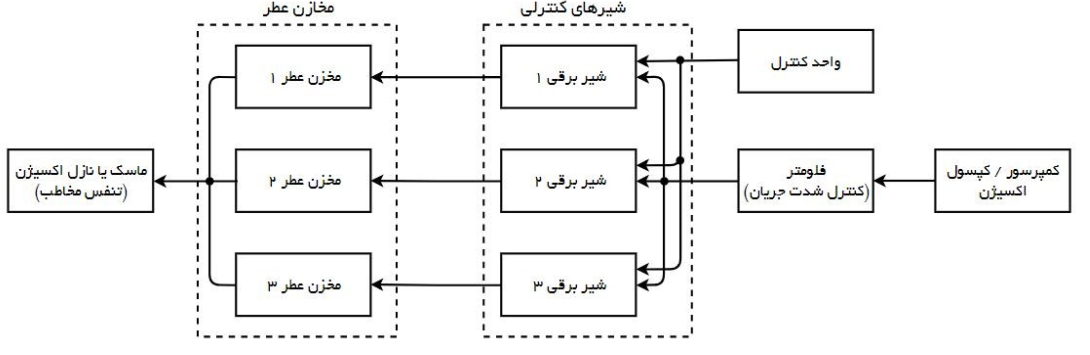
\includegraphics[width=1\textwidth]{sche.png}
	\caption{شماتیک دستگاه}
	\label{fig:sche1}
\end{figure}

جریان هوا به سه شاخه تقسیم می‌شود و هر شاخه به یک شیر سلونوییدی وصل می گردد؛ شیر سلونوییدی را به کمک جریان برق می‌توان قطع و وصل نمود و این ویژگی به ما این امکان را می‌دهد تا بوهایی که به آزمایش‌شونده می‌رسد را کنترل کنیم. به منظور کنترل‌کردن شیر نیز از آردوینو استفاده می کنیم. آردوینو یک برد مبتنی بر میکروکنترلر AVR است که می‌توان آن را به کمک کامپیوتر برنامه‌ریزی کرد و خروجی‌های آن را کنترل نمود.

\begin{figure}[h]
	\centering
	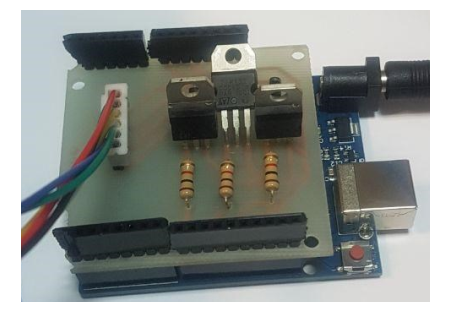
\includegraphics[width=0.4\textwidth]{arduino.png}
	\caption{مدار کنترلی}
	\label{fig:sche1}
\end{figure}


از آنجایی که ولتاژ خروجی آردوینو 5 ولت و ولتاژ مورد نیاز برای باز شدن شیر 12 ولت است، از مدار دیگری استفاده می‌کنیم که به کمک ورودی 5 ولت، منبع 12 ولتی را قطع و وصل می‌کند.


خروجی شیرها را وارد ظرفی می‌کنیم که تا نیمه با اسانس محلول پر شده‌است. با باز شدن شیر، جریان هوا باعث می‌شود تا هوای بالای ظرف عطر آگین شود و این هوا به بینی آزمایش‌شونده می‌رسد.
هر بار فقط یکی از شیرها باز می شود و سایر شیرها بسته می‌باشند تا تمامی جریان هوا از یکی از ظرف‌ها بگذرد و هوای خروجی حامل بوی ظرف مورد نظر باشد. تمامی لوله‌هایی که از ظرف خارج می‌شوند به یکدیگر متصل می‌شوند و جریان هوا در نهایت به کمک یک ماسک اکسیژن به آزمایش‌شونده می‌رسد.
شکل ۳، تصویری از صورت نهایی دستگاه است.
\begin{figure}[h]
	\centering
	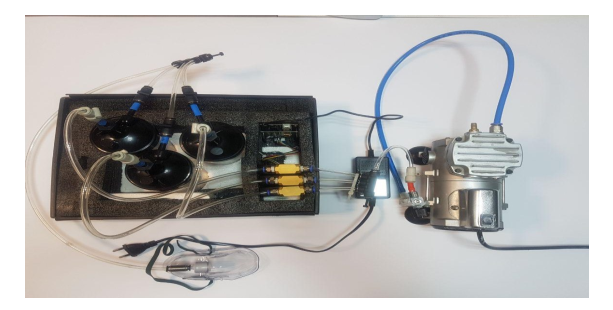
\includegraphics[width=1\textwidth]{full.png}
	\caption{تصویر نهایی دستگاه}
	\label{fig:sche1}
\end{figure}


%%%%%%%%%%%%% مراجع %%%%%%%%%%%%%%%%%%%%%%%%%%%%%
\begin{thebibliography}{9}
\begin{latin}


 \bibitem{Lorig}
 Tyler S. Lorig. \textrm{The application of electroencephalographic techniques to the study of human olfaction: a review and tutorial}, \textbf{International Journal of Psychophysiology},  (36)  91–104, 2000.

\bibitem{Elmes}
Tyler S. Lorig , David G. Elmes. \textrm{A computer-controlled olfactometer for fMRI and electrophysiological studies of olfaction}, \textbf{Behavior Research Methods, Instruments, \& Computers} 31 (2), 370–375, 1999.

\bibitem{Lunder}
Johan N. Lundström. \textrm{Methods for building an inexpensive computer-controlled olfactometer for temporally – precise experiments}, \textbf{International Journal of Psychophysiology},  (78) 179 – 189, 2010.

\bibitem{Kroupi}
Eleni Kroupi.  \textrm{EEG Correlates of Pleasant and Unpleasant Odor Perception},  \textbf{ACM Trans. Multimedia Comput. Commun. Appl.}, (11), 2014.

\bibitem{Lowen}
Steven B. Lowen, Scott E. Lukas. \textrm{A low – cost, MR-compatible olfactometer},  \textbf{Behavior Research Methods}, 38 (2) 307-313, 2006. 

\end{latin}
\end{thebibliography}
\newpage
  \thispagestyle{empty} 
  \setcounter{footnote}{0} 
 \end{document}
